
% Figure inclusion code for report.tex

% Figure 1: Dataset Overview
\begin{figure}[htbp]
\centering
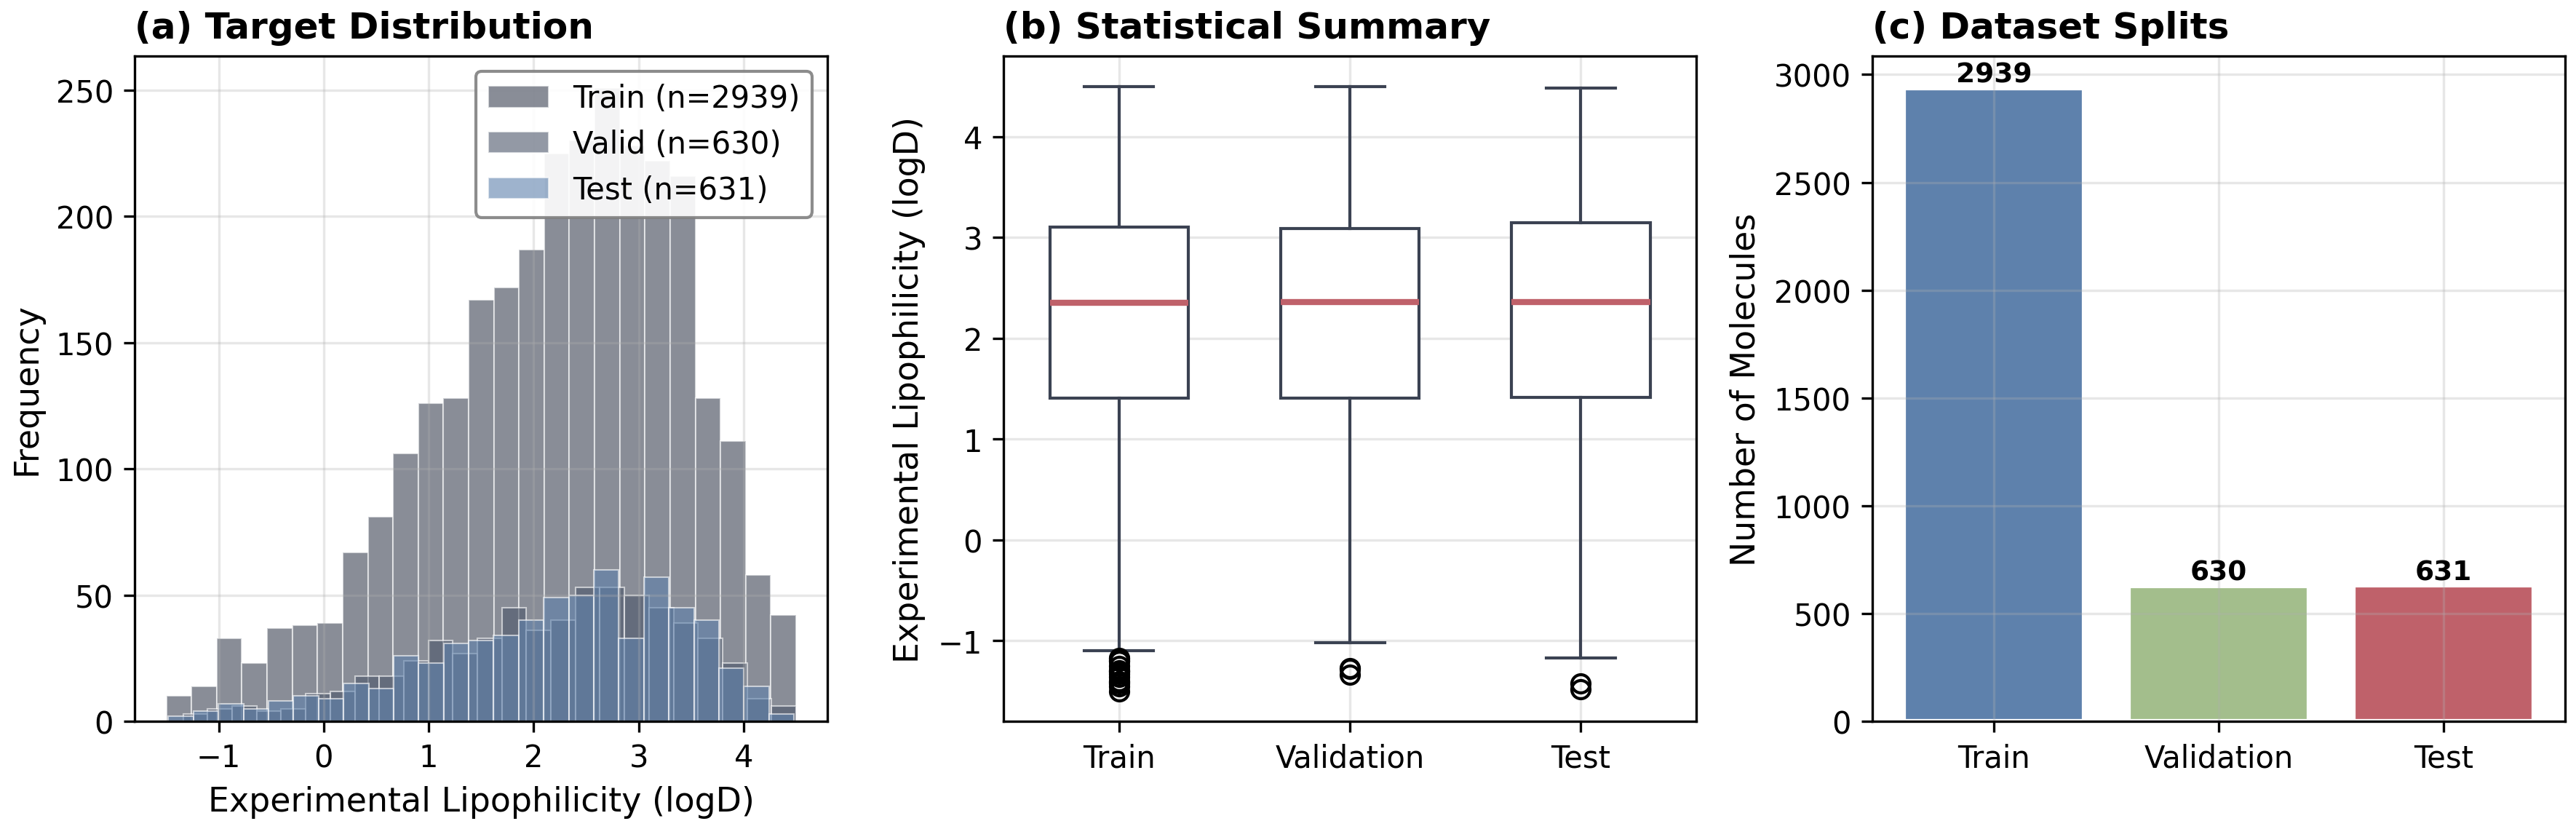
\includegraphics[width=0.95\textwidth]{figures/professional/fig1_dataset_overview.png}
\caption{Dataset overview. (a) Target value distribution across train, validation, and test sets. (b) Statistical summary by split. (c) Sample sizes.}
\label{fig:dataset_overview}
\end{figure}

% Figure 2: Chemical Space Analysis
\begin{figure}[htbp]
\centering
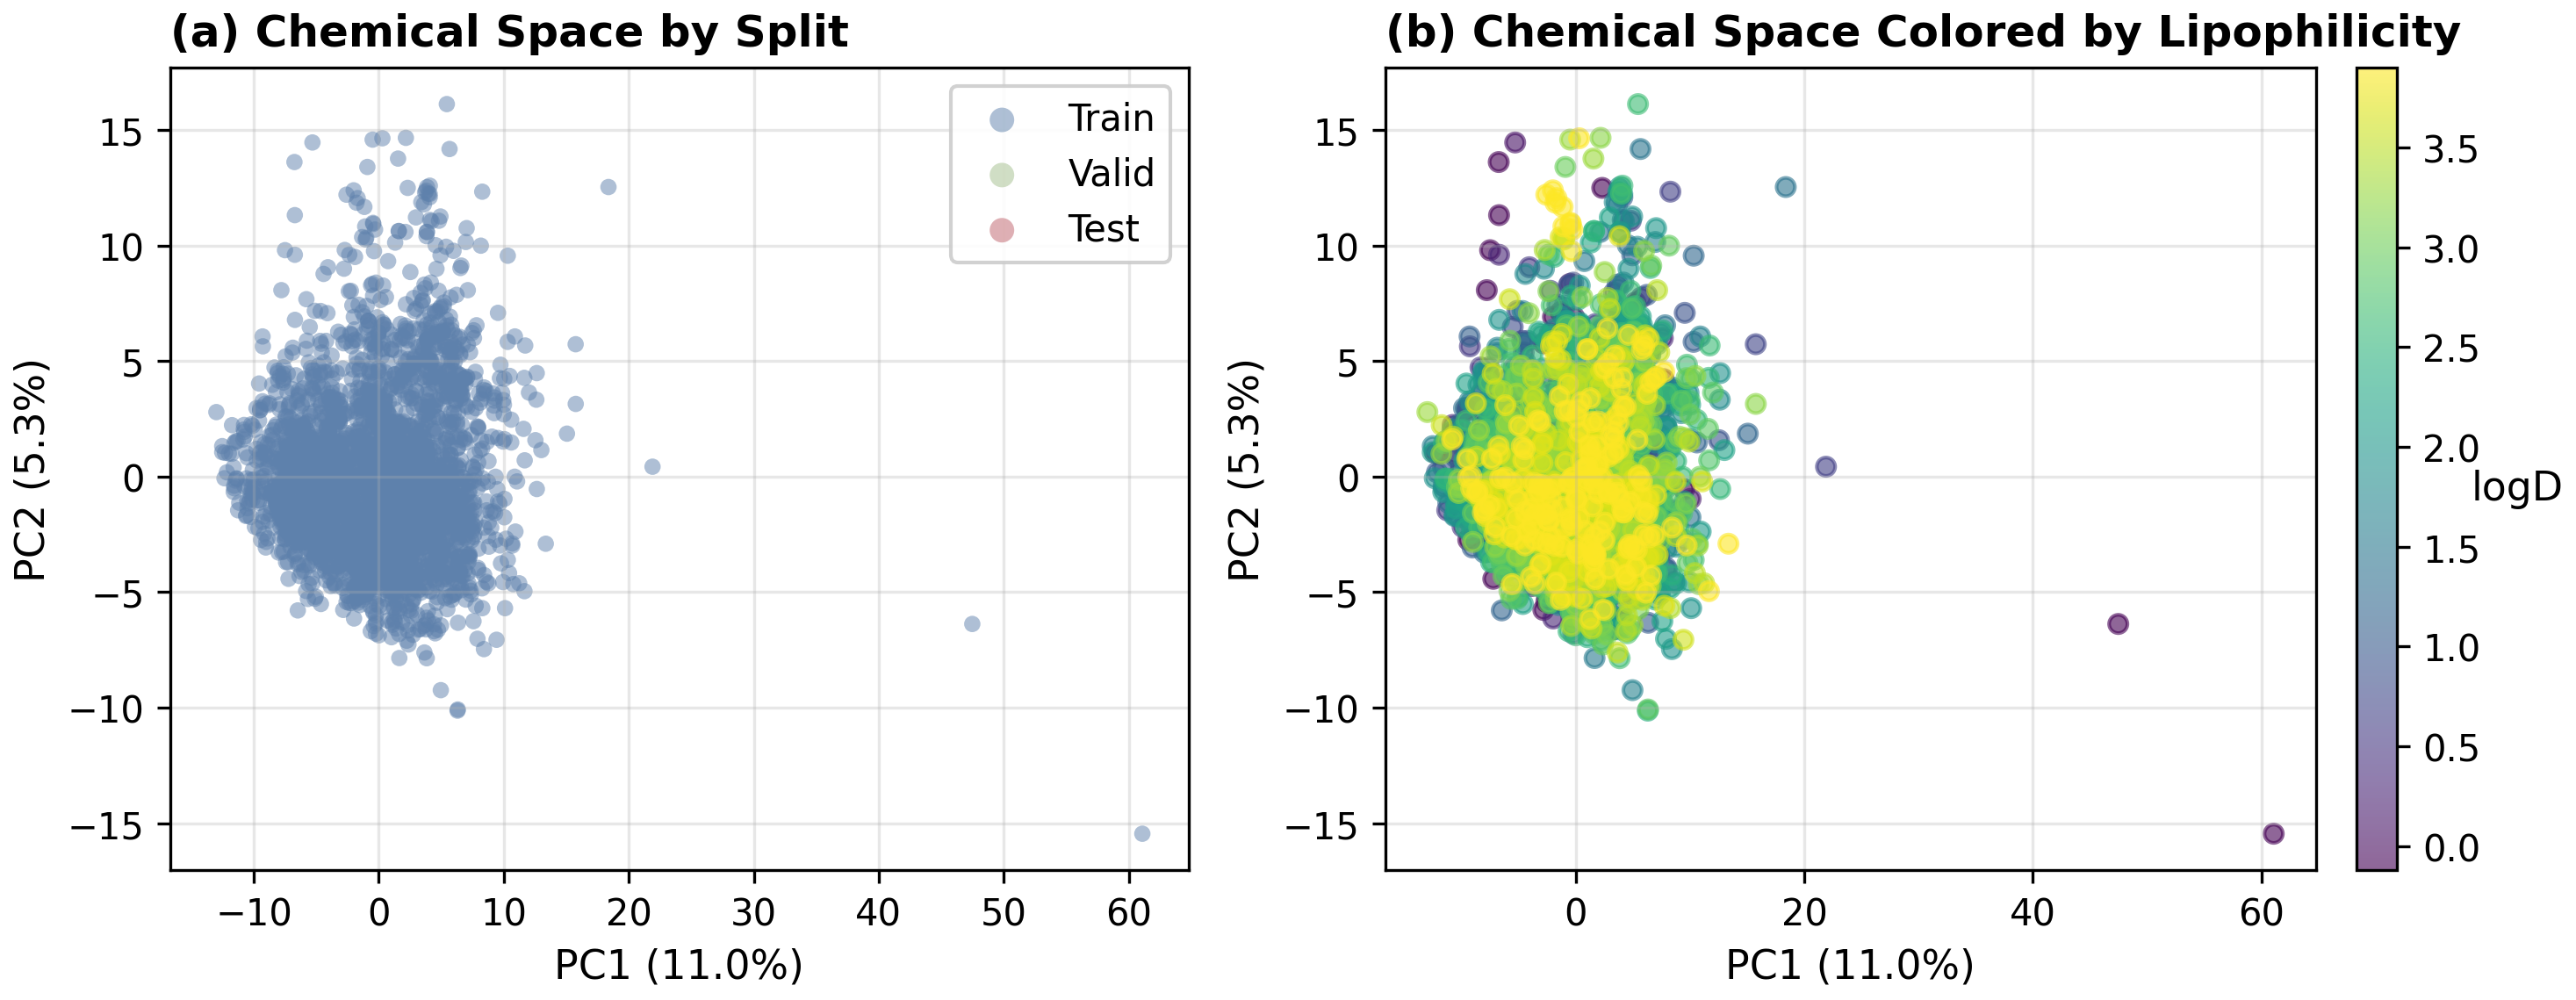
\includegraphics[width=0.95\textwidth]{figures/professional/fig2_chemical_space.png}
\caption{Chemical space analysis. (a) PCA projection colored by dataset split. (b) PCA projection colored by lipophilicity value.}
\label{fig:chemical_space}
\end{figure}

% Figure 3: Model Performance
\begin{figure}[htbp]
\centering
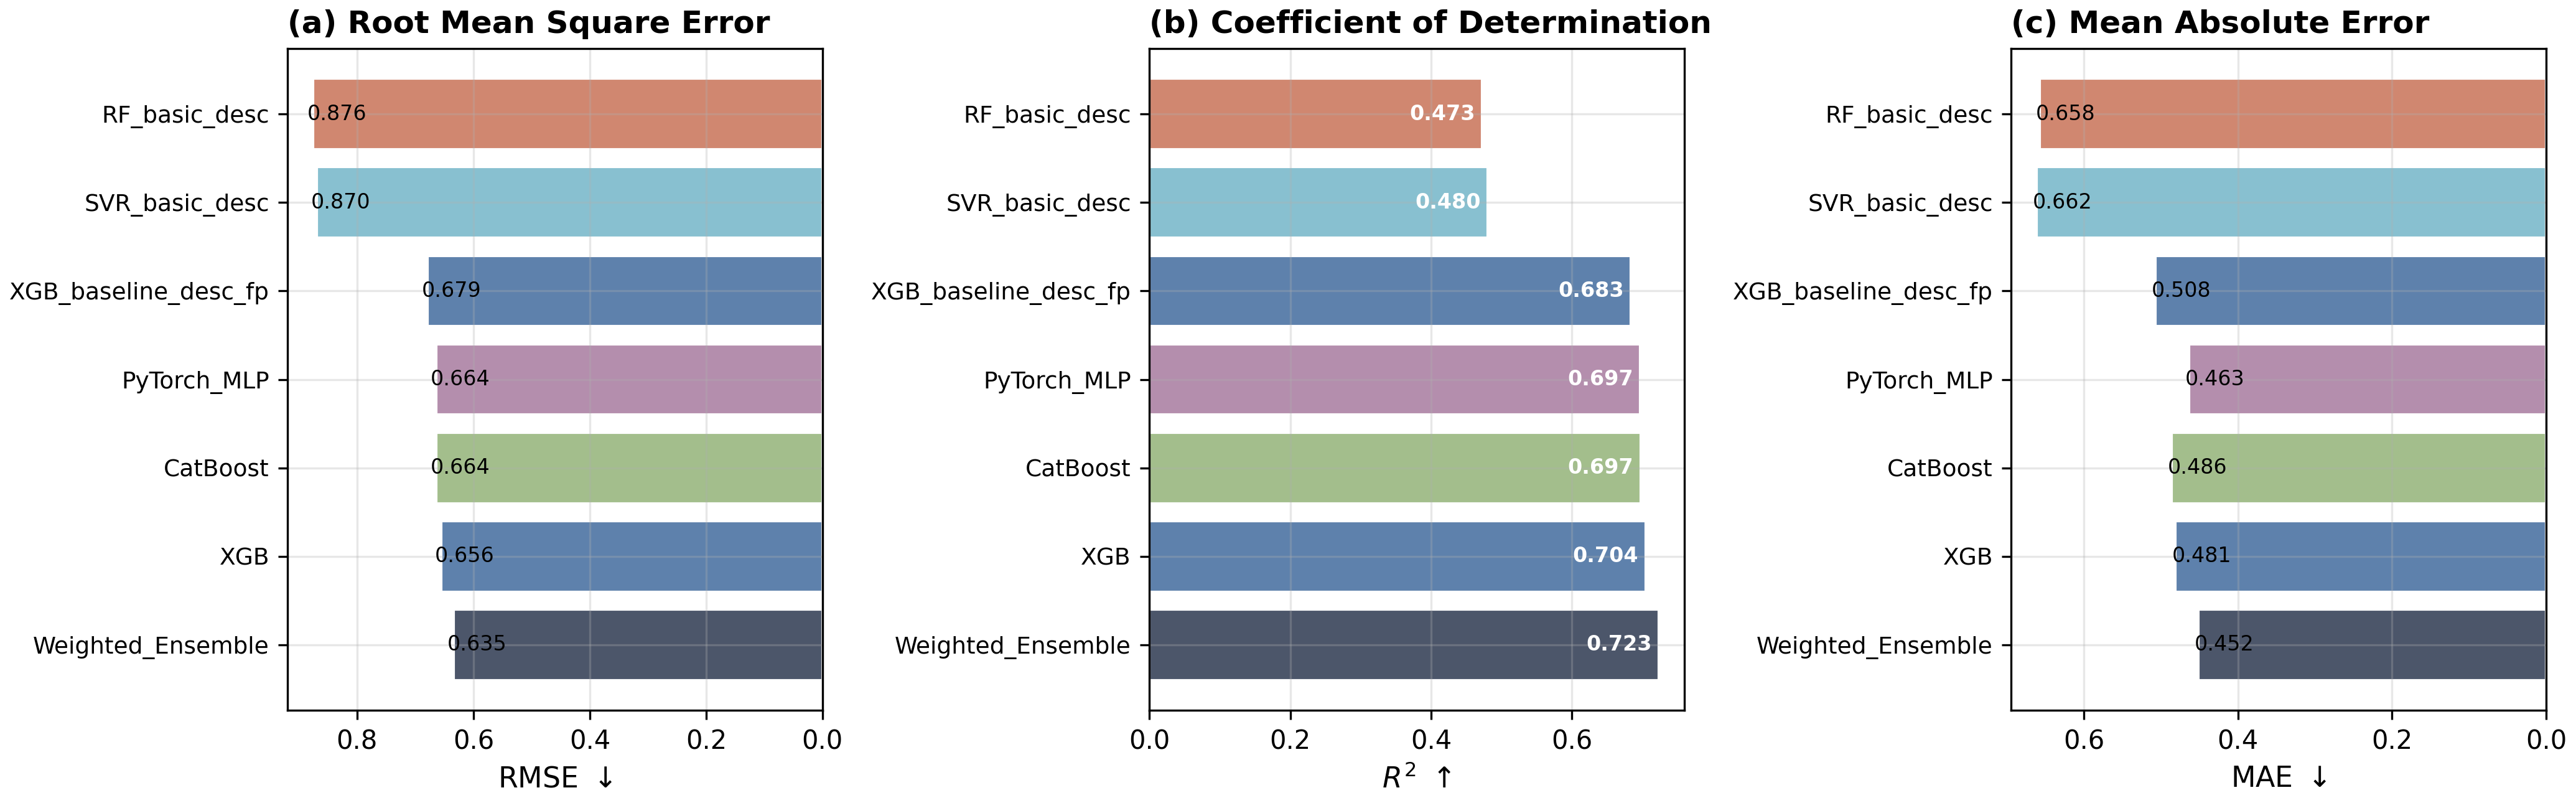
\includegraphics[width=0.95\textwidth]{figures/professional/fig3_model_performance.png}
\caption{Model performance comparison. (a) Root Mean Square Error (lower is better). (b) Coefficient of Determination $R^2$ (higher is better). (c) Mean Absolute Error (lower is better).}
\label{fig:model_performance}
\end{figure}

% Figure 4: Prediction vs Observation
\begin{figure}[htbp]
\centering
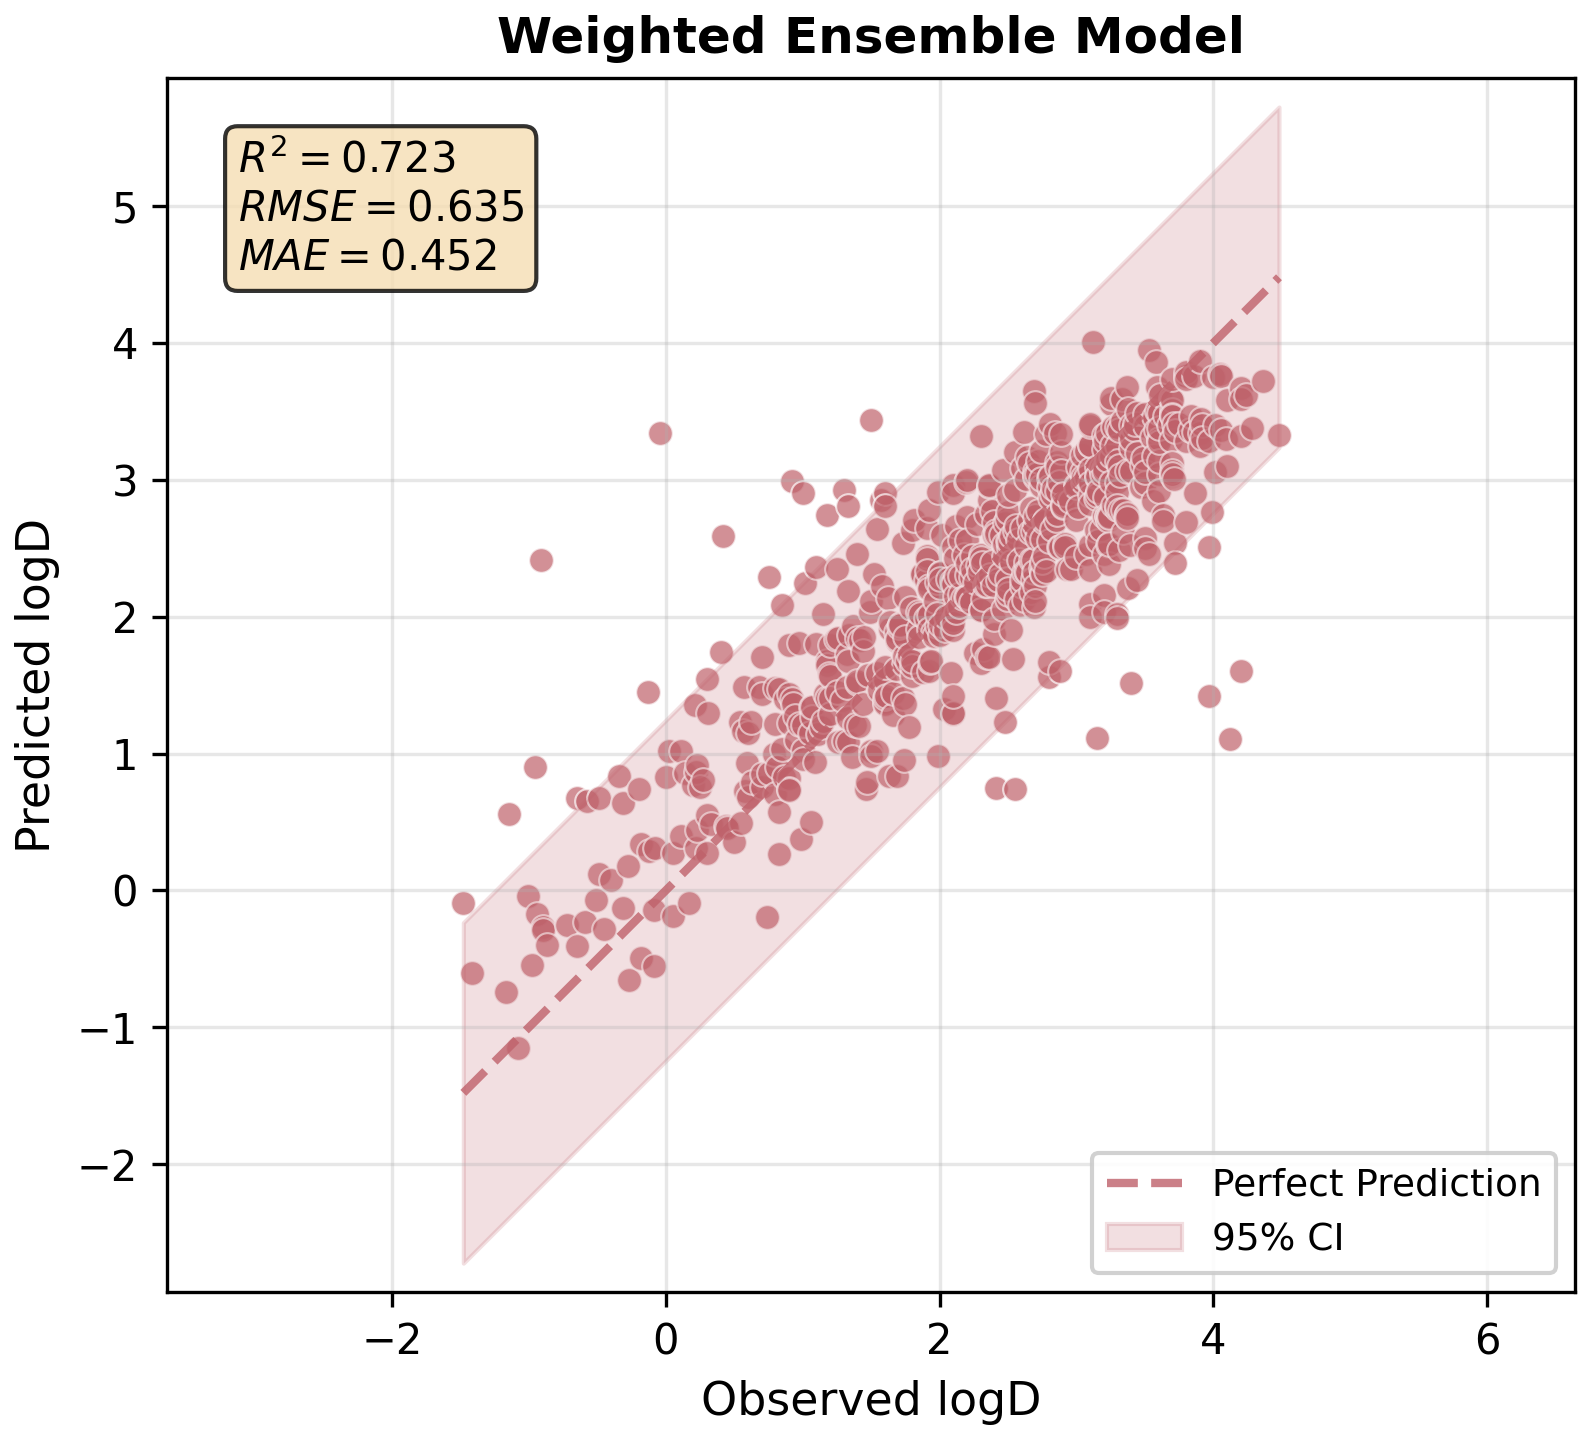
\includegraphics[width=0.65\textwidth]{figures/professional/fig4_ensemble_prediction_scatter.png}
\caption{Predicted versus observed lipophilicity for the ensemble model. The diagonal red line represents perfect prediction. The shaded region indicates the 95\% confidence interval. Metrics: $R^2 = 0.723$, RMSE $= 0.635$, MAE $= 0.452$.}
\label{fig:prediction_scatter}
\end{figure}

% Figure 5: Residual Analysis
\begin{figure}[htbp]
\centering
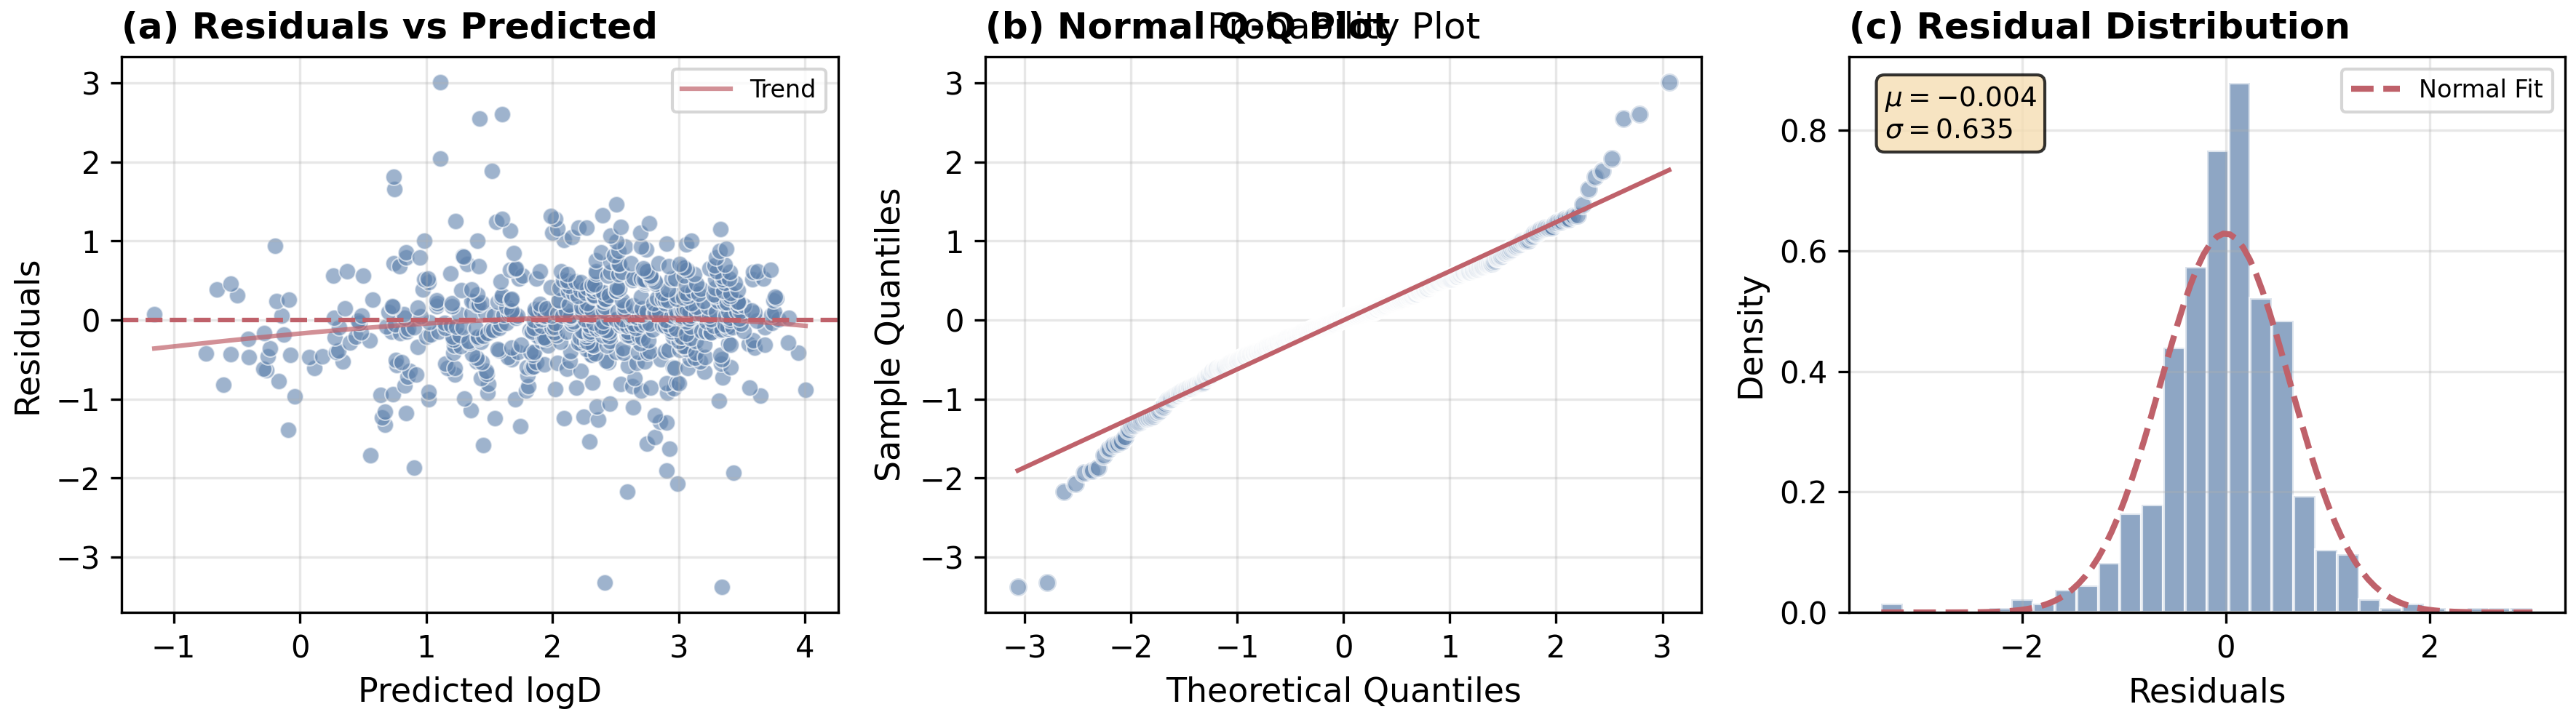
\includegraphics[width=0.95\textwidth]{figures/professional/fig5_residual_analysis.png}
\caption{Residual analysis for the ensemble model. (a) Residuals versus predicted values with LOESS trend line. (b) Normal Q-Q plot. (c) Residual distribution with normal fit.}
\label{fig:residuals}
\end{figure}

% Figure 6: Feature Importance
\begin{figure}[htbp]
\centering
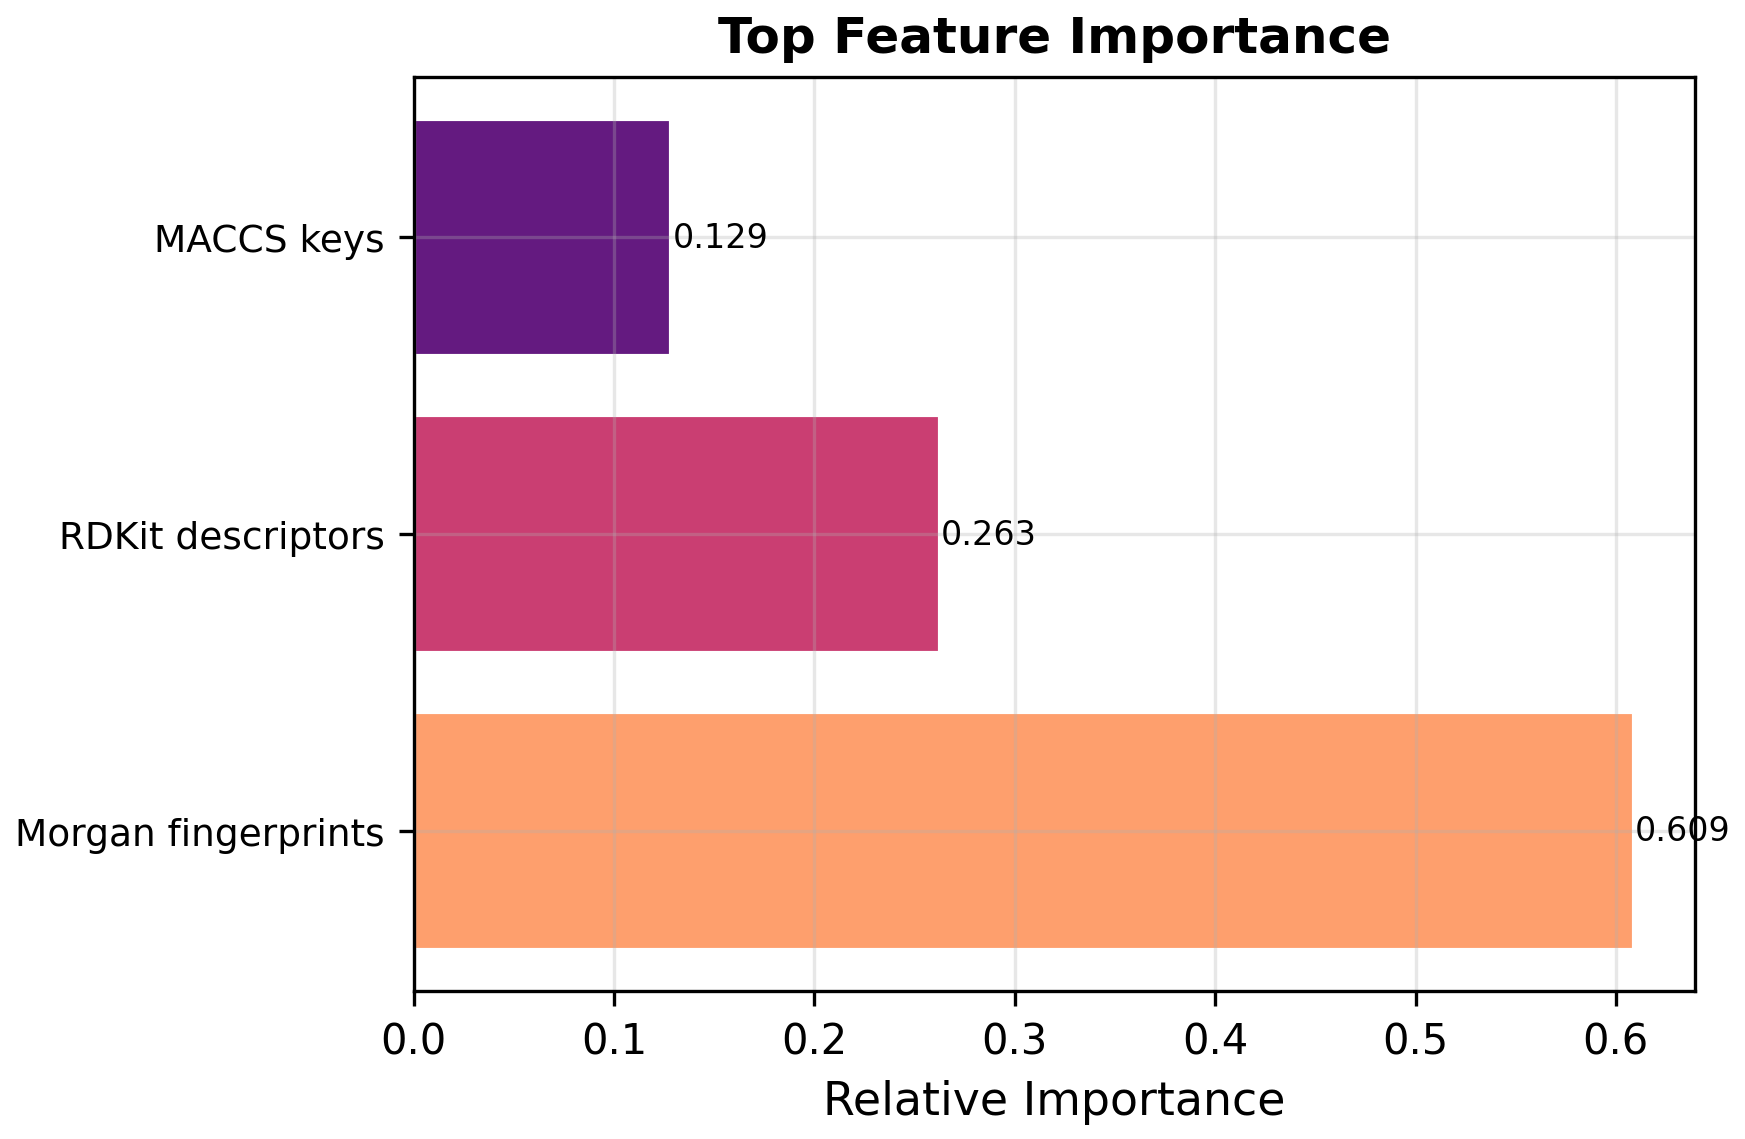
\includegraphics[width=0.7\textwidth]{figures/professional/fig6_feature_importance.png}
\caption{Feature importance by family in the enhanced XGBoost model. All three feature families contribute significantly to model predictions.}
\label{fig:feature_importance}
\end{figure}

% Figure 7: Ensemble Weights
\begin{figure}[htbp]
\centering
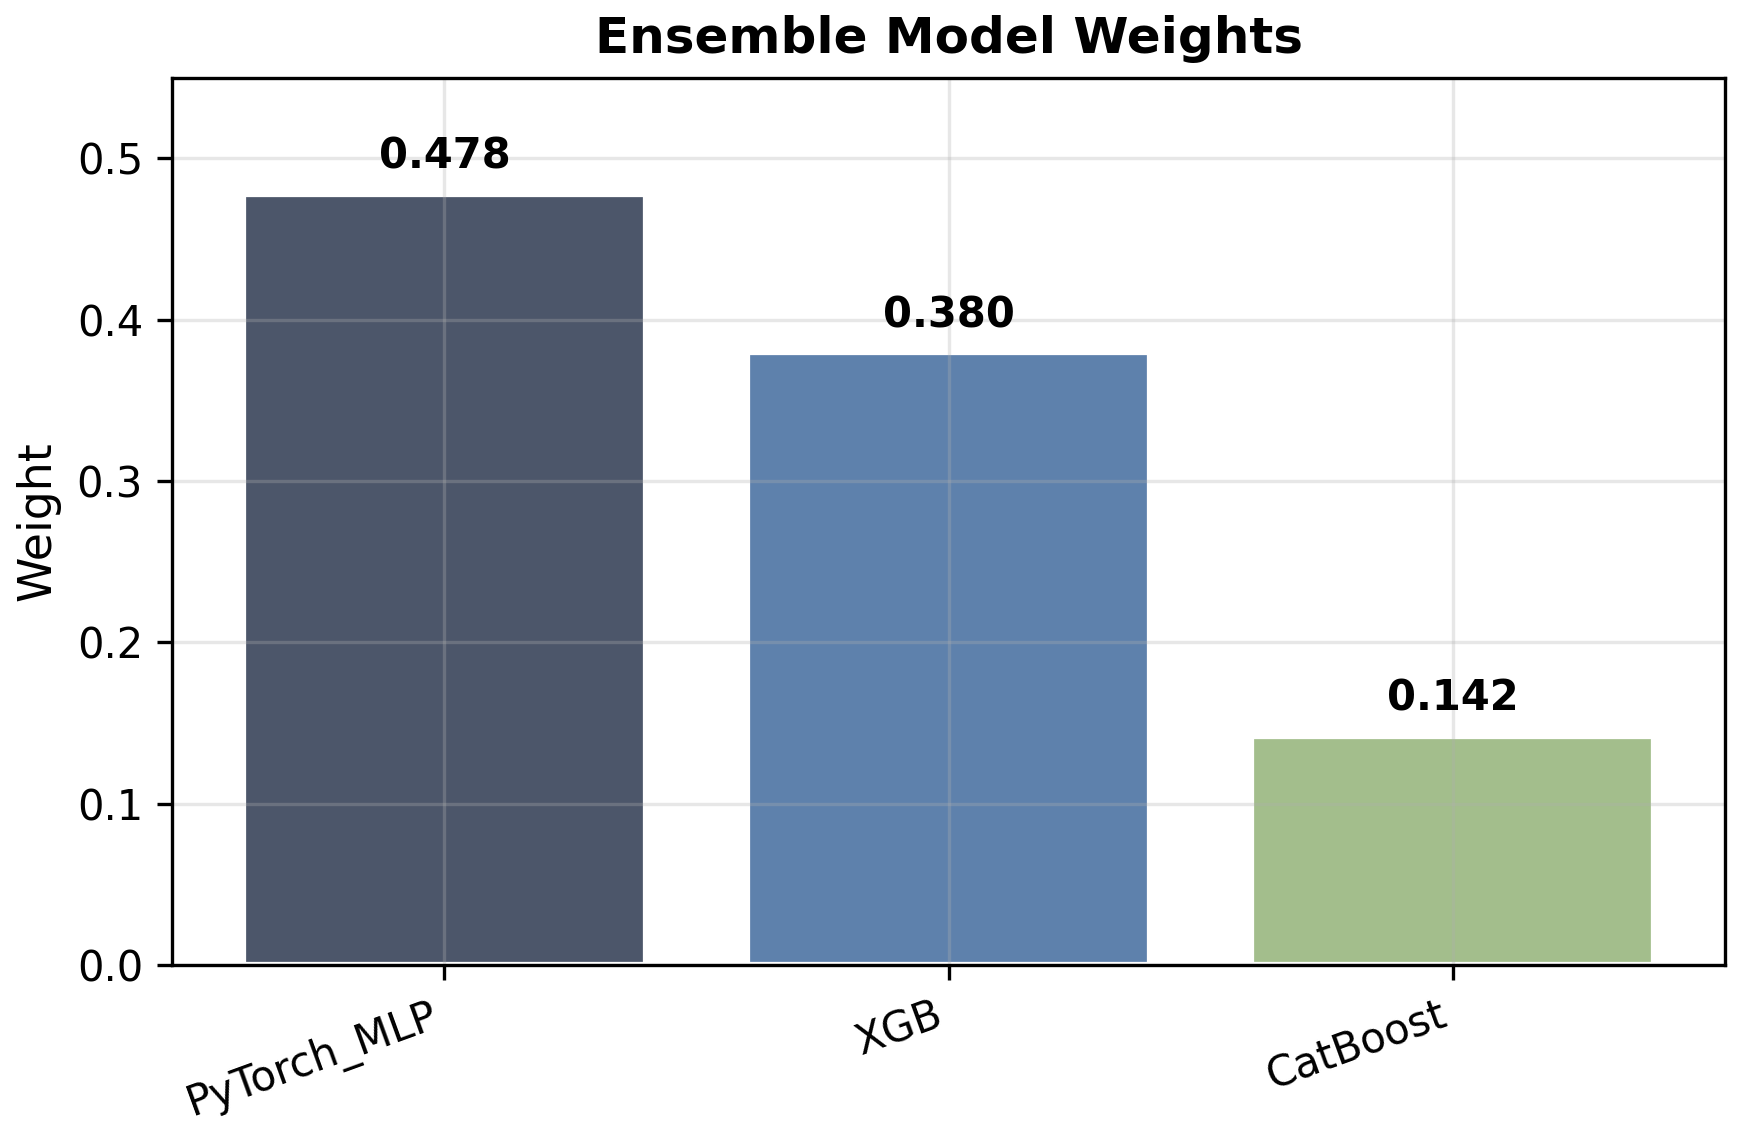
\includegraphics[width=0.65\textwidth]{figures/professional/fig7_ensemble_weights.png}
\caption{Optimal ensemble weights for combining XGBoost, CatBoost, and PyTorch MLP predictions.}
\label{fig:ensemble_weights}
\end{figure}

% Figure 8: Scaffold Analysis
\begin{figure}[htbp]
\centering
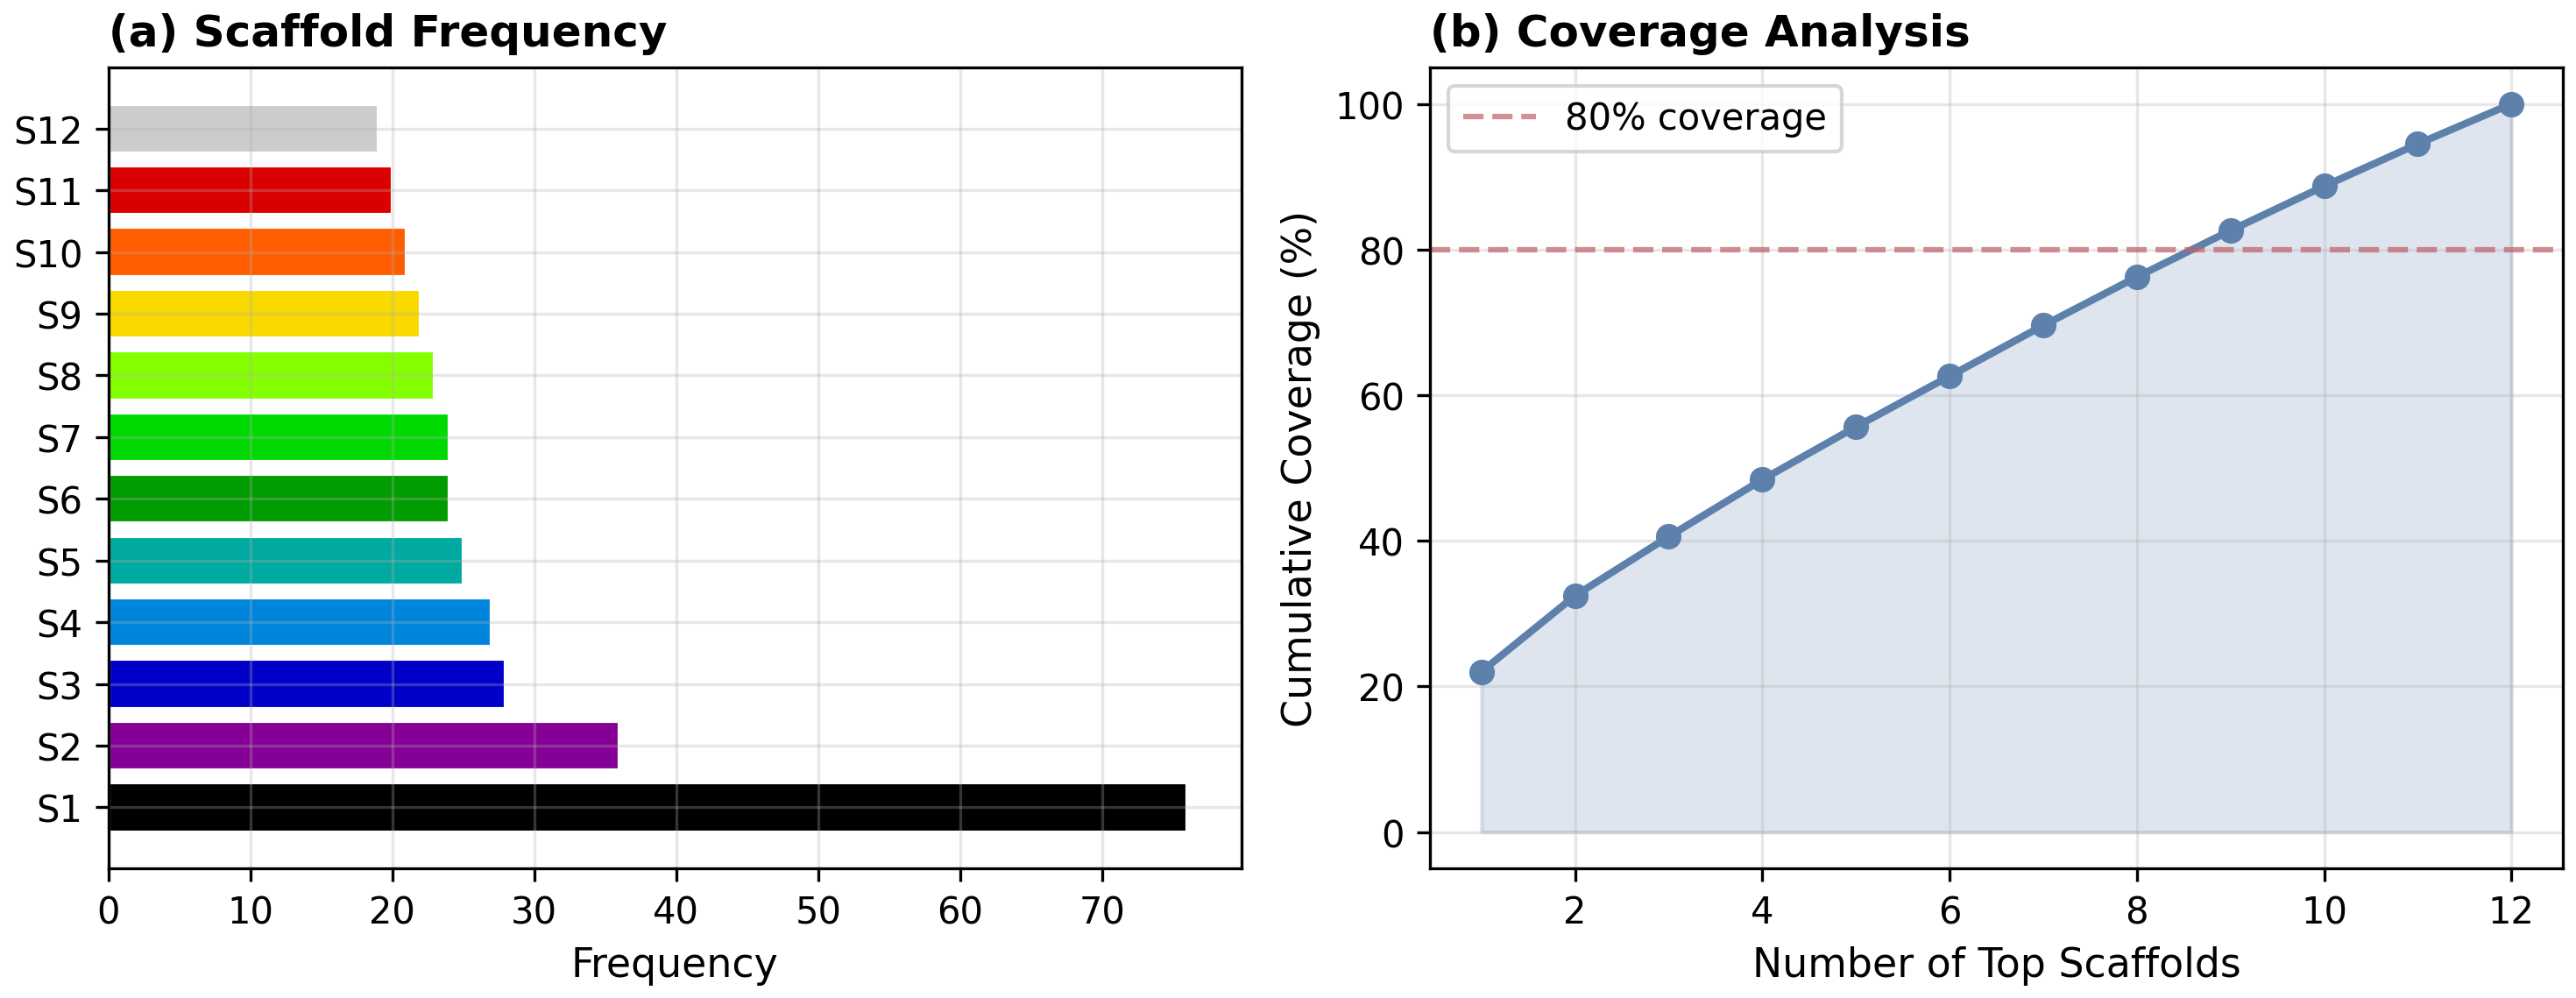
\includegraphics[width=0.95\textwidth]{figures/professional/fig8_scaffold_analysis.png}
\caption{Scaffold analysis. (a) Frequency of top 12 Bemis--Murcko scaffolds. (b) Cumulative coverage of molecular space by top scaffolds.}
\label{fig:scaffold}
\end{figure}
